%% This is an example first chapter.  You should put chapter/appendix that you
%% write into a separate file, and add a line \include{yourfilename} to
%% main.tex, where `yourfilename.tex' is the name of the chapter/appendix file.
%% You can process specific files by typing their names in at the 
%% \files=
%% prompt when you run the file main.tex through LaTeX.
\chapter{Specification}

The following section describes what the system does detailing its features.

\section{Uses Case Model}

This section describes the services of the systems as events triggered by external actors and their interrelation.

\subsection*{Actors}

The actors of the system are:

\begin{description}
	\item[Sensor device] The device responsible for registering itself in the system and sending the gathered observations to it. As the design and building of the sensor device is out of the scope of the project, it is simulated by a CLI tool that allows to issue request against the system.
	\item[Web application user] A person who interacts with the public web application that shows the observations in a data visualization.
\end{description}

\subsection{Use Cases}

\begin{figure}[h]
	\centering
	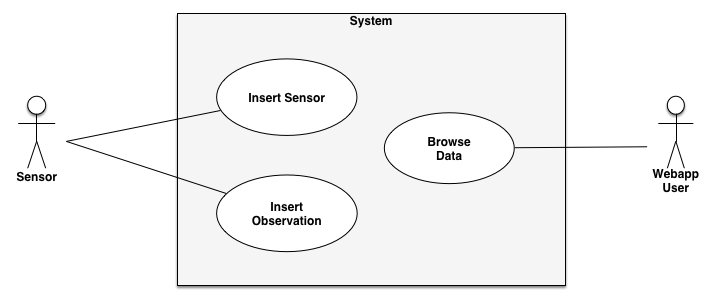
\includegraphics[width=\textwidth]{uses_cases}
	\caption{System's use cases}
	\label{fig:use_cases}
\end{figure}

\begin{usecase}
	\addtitle{Use Case 1}{Insert Sensor}
	\addfield{Actors:}{Sensor device}
	\addfield{Preconditions:}{The system is running}
	\addfield{Postconditions:}{The sensor is registered and persisted in the system}
	\addscenario{Main Success Scenario:}{
		\item The sensor issues a POST request to the sensors endpoint
		\item The system stores the sensor's information in the database
		\item The system sends a HTTP response with 201 status code to the sensor
	}
\end{usecase}

\begin{usecase}
	\addtitle{Use Case 2}{Insert Observation}
	\addfield{Actors:}{Sensor device}
	\additemizedfield{Preconditions:}{
		\item The system is running
		\item The sensor is registered in the system	
	}
	\additemizedfield{Postconditions:}{
		\item The observation is persisted in the system
		\item The observation is sent to the web application tier
	}
	\addscenario{Main Success Scenario:}{
		\item The sensor issues a POST request to the observations endpoint
		\item The system stores the observation's data in the database
		\item The system sends the observation's data to the web application tier
		\item The system sends a HTTP response with 201 status code to the sensor
	}
\end{usecase}

\section{Conceptual Model}
